\begin{question}\vspace*{-20pt}
\begin{instance}  
\begin{statement}
\parbox{200pt}{\raggedright 

\begin{center}
	
\includegraphics[width=0.3\textwidth]{NonQuestions/Figure_Slide_6a.jpg}
\end{center}
	
Juan es embajador y Luisa es una cantante de ópera famosa. La radio española difunde sus canciones. 
	
	}\hspace*{2cm}\parbox{200pt}{\raggedright 

\begin{center}
	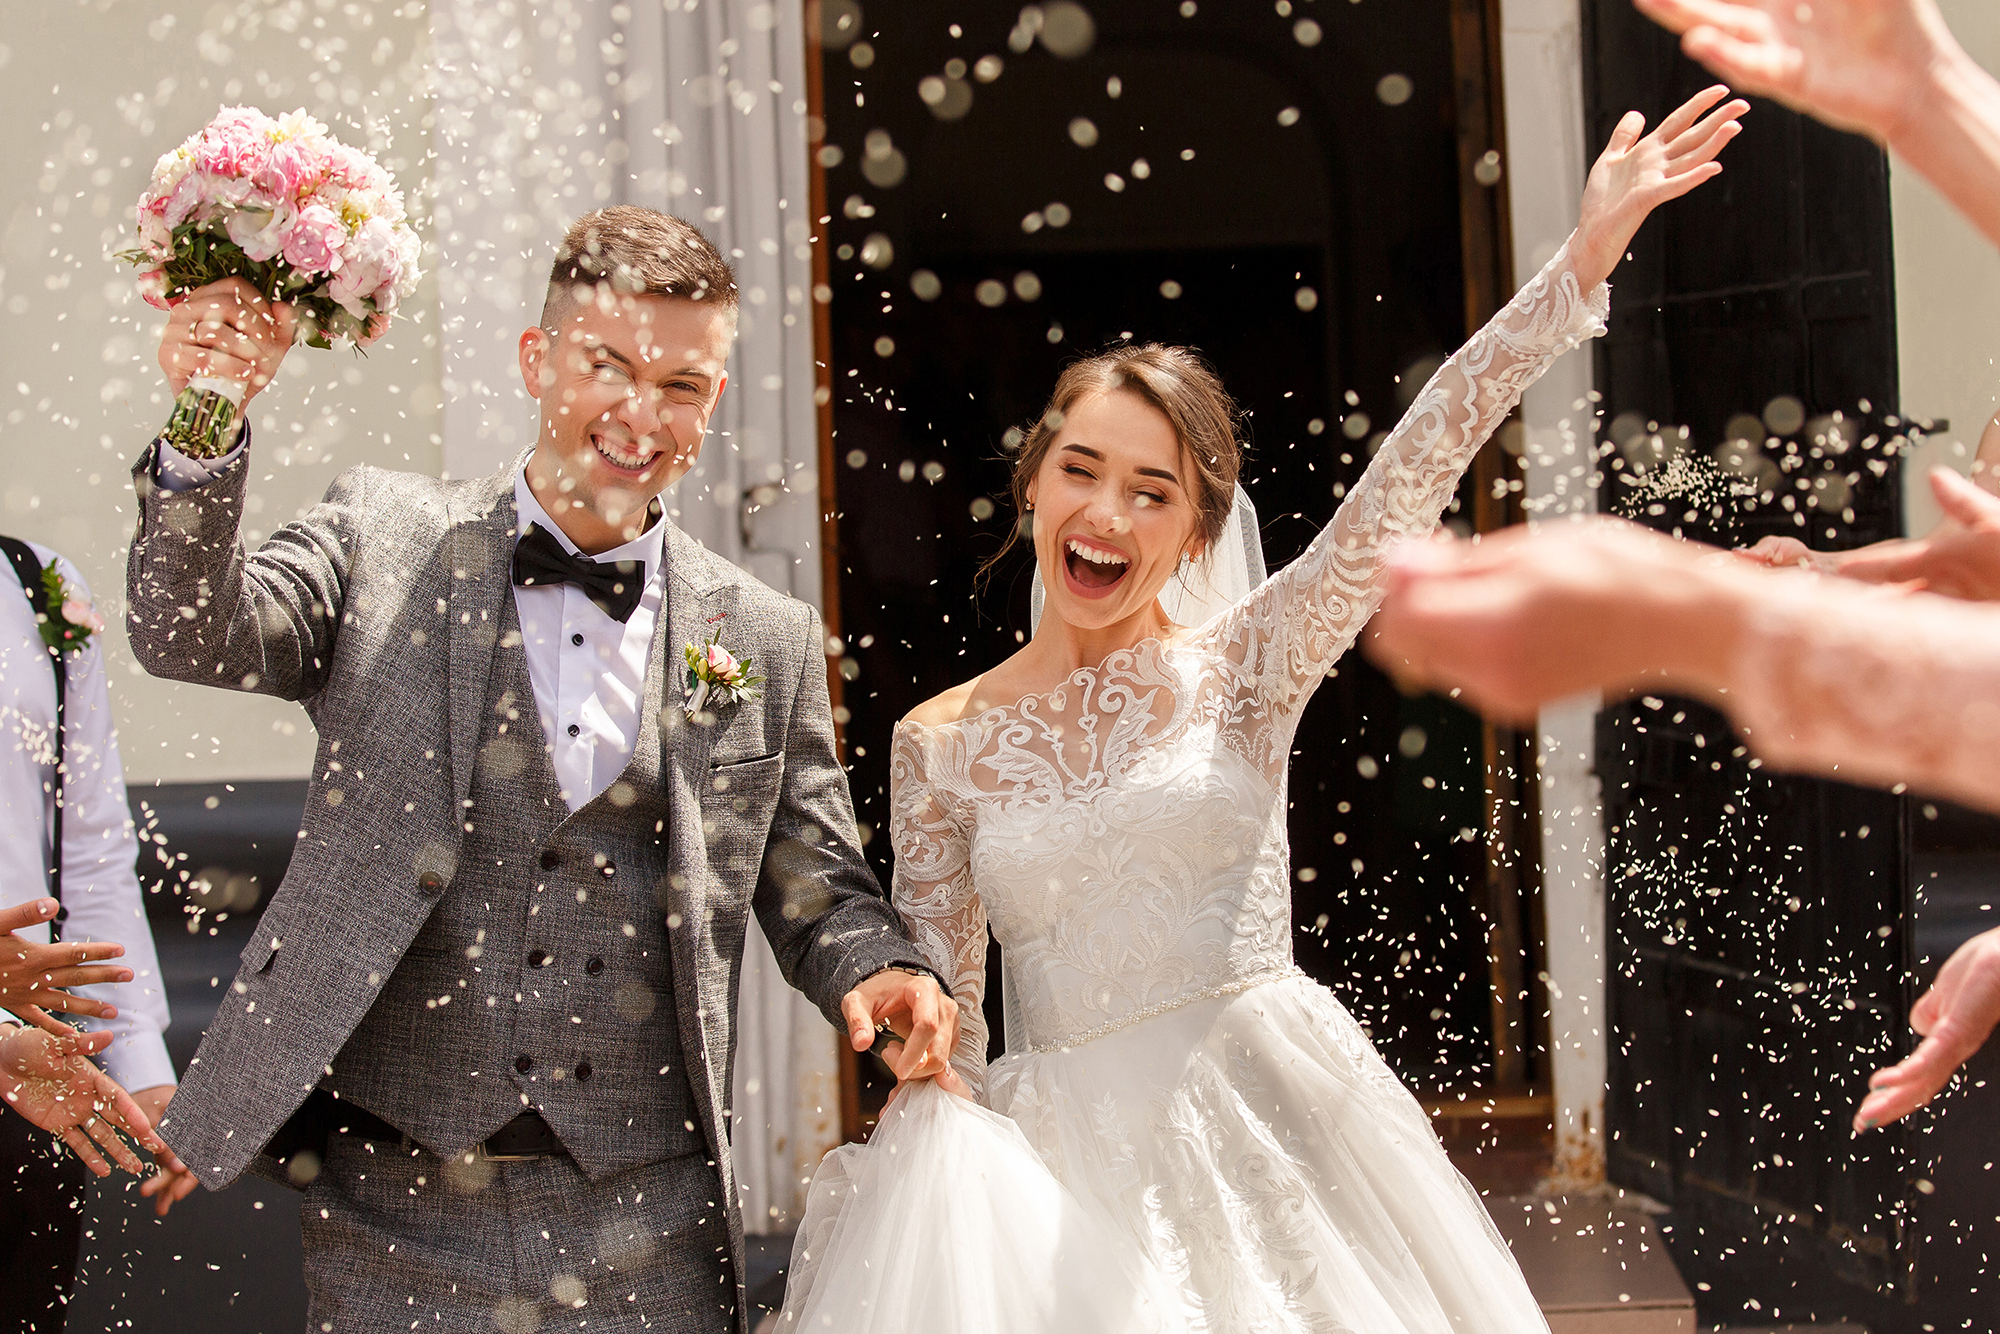
\includegraphics[width=0.3\textwidth]{NonQuestions/Figure_Slide_6b.jpg}
\end{center}
	
El mes pasado Juan y su mujer asistieron a la boda de su nieto. \vspace*{60pt}
	
	}\hspace*{2cm}\parbox{200pt}{\raggedright 

\begin{center}
	
\includegraphics[width=0.3\textwidth]{NonQuestions/Figure_Slide_6c.jpg}
\end{center}
	
A Luisa le encanta leer biografías con su marido Juan. \vspace*{60pt}
	
	}\vspace*{40pt}
\end{statement} 
\begin{mcq}[standalone=true,no-label=true]      
\begin{stem}
Elige la opción correcta.

\end{stem}    
\begin{distractors}
\distractor{Los textos hablan de la vida personal y profesional de dos personas casadas.}
\distractor{Los textos hablan de los gustos y preferencias de dos personas casadas.}
\distractor{Las dos opciones son correctas.}
\end{distractors}
\end{mcq}
\end{instance}
\end{question}